%\documentclass[a4paper]{article}
\usepackage[utf8]{inputenc}
\usepackage[spanish, es-tabla, es-noshorthands]{babel}
\usepackage[table,xcdraw]{xcolor}
\usepackage[a4paper, footnotesep=1.25cm, headheight=1.25cm, top=2.54cm, left=2.54cm, bottom=2.54cm, right=2.54cm]{geometry}
%\geometry{showframe}

%\usepackage{wrapfig}			%Wrap figure in text
\usepackage[export]{adjustbox}	%Move images
\usepackage{changepage}			%Move tables

\usepackage{tikz}
\usepackage{amsmath}
\usepackage{amsfonts}
\usepackage{amssymb}
\usepackage{float}
\usepackage{graphicx}
\usepackage{caption}
\usepackage{subcaption}
\usepackage{multicol}
\usepackage{multirow}
\usepackage{wrapfig}
\setlength{\doublerulesep}{\arrayrulewidth}
\usepackage{booktabs}
\usepackage[numbib, nottoc, notlot, notlof]{tocbibind}

\usepackage{hyperref}
\hypersetup{
    colorlinks=true,
    linkcolor=blue,
    filecolor=magenta,      
    urlcolor=blue,
    citecolor=blue,    
}

%Change Font Size

% #1 = size, #2 = text
\newcommand{\setparagraphsize}[2]{{\fontsize{#1}{6}\selectfont#2 \par}}		%Cambia el size de todo el parrafo
\newcommand{\setlinesize}[2]{{\fontsize{#1}{6}\selectfont#2}}				%Cambia el font de una oración

\newcommand{\note}[1]{
	\begin{center}
		\huge{ \textcolor{red}{#1} }
	\end{center}
}

%FONTS (IMPORTANTE): Compilar en XeLaTex o LuaLaTeX
\usepackage{anyfontsize}	%Font size
\usepackage{fontspec}		%Font type

\usepackage{etoolbox}
\usepackage{todonotes}

\newcommand{\observacion}[2]{  \ifnumequal{1}{#1}{ { \todo[inline,backgroundcolor=red!25,bordercolor=red!100]{\textbf{Observación: #2}} } }{  }  }

\setcounter{topnumber}{2}
\setcounter{bottomnumber}{2}
\setcounter{totalnumber}{4}
\renewcommand{\topfraction}{0.85}
\renewcommand{\bottomfraction}{0.85}
\renewcommand{\textfraction}{0.15}
\renewcommand{\floatpagefraction}{0.8}
\renewcommand{\textfraction}{0.1}
\setlength{\floatsep}{5pt plus 2pt minus 2pt}
\setlength{\textfloatsep}{5pt plus 2pt minus 2pt}
\setlength{\intextsep}{5pt plus 2pt minus 2pt}

\newcommand{\quotes}[1]{``#1''}
\usepackage{array}
\newcolumntype{C}[1]{>{\centering\let\newline\\\arraybackslash\hspace{0pt}}m{#1}}
\usepackage[american]{circuitikz}
\usetikzlibrary{calc}
\usepackage{fancyhdr}
\usepackage{units} 

\graphicspath{{../Control de posición no lineal/}{../Control de fuerza no lineal/}{../Control híbrido no lineal/}{../Referencias/}{../Deducción de modelo/}{../Conclusiones/}}

\pagestyle{fancy}
\fancyhf{}
\lhead{22.99 - Automación Industrial}
\rhead{Lambertucci, Londero B., Maselli, Mechoulam}
\rfoot{Página \thepage}

%Items con bullets y no cuadrados
\renewcommand{\labelitemi}{\textbullet }


%\begin{document}

\subsection{Caracterizaci\'on del problema}
Se pide un control cartesiano no lineal para el manipulador RR. Agregando una zona prohibida que es todo valor por encima de una pared, descrita en el plano XY pro la siguiente ecuaci\'on:
\begin{equation}
y=2-x
\end{equation}
Al manipulador se le pide que vaya del punto (1;-1;0) a (1;1;0). Para generar la trayectoria se utiliza la función \textbf{jtraj} del toolbox de matlab de Peter Corke.
\subsection{Esquema de control}
El modelo de control porpuesto es el conocido como linealizaci\'on por realimentaci\'on.
Es fundamental para este tipo de control tener un gran conocimiento de la planta, ya que basicamente se lo controla como si fuese lineal, con un esquema tipo PD. Con la diferencia que se le agrega  a la acci\'on de control la respuesta no lineal de la planta, gracias al conocimiento del modelo no lineal de la planta y sus variables de estado.
\begin{figure}[H]
	\centering
	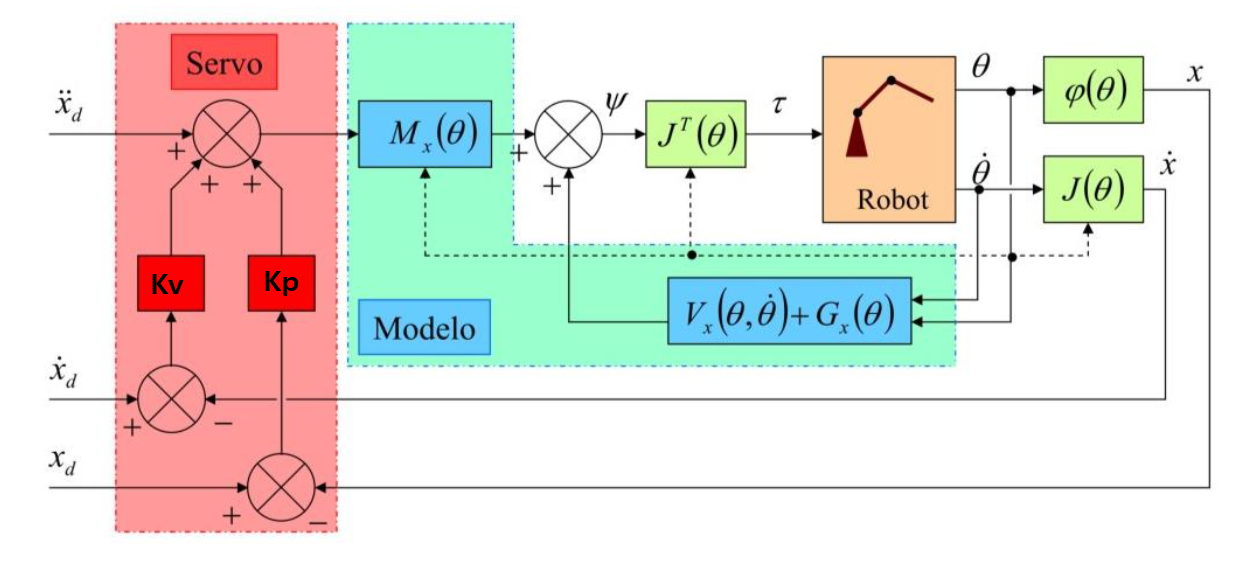
\includegraphics[width=0.8\linewidth]{ImagenesControl de posición no lineal/modelo_control_p}
	\caption{Topolog\'ia del control de posici\'on cartesiano no lineal.}	
	\label{fig:control_p_modelo}
\end{figure}
Cabe mencionar que las matrices $M_x,\ V_x, \ y \ G_x$ se encuentran en espacio cartesiano, y la manera de pasar de las mismas en espacio joint es la siguiente:
\begin{equation}
M_x(\Theta) = J^{-T}(\Theta) M(\Theta) J^{-1}(\Theta)
\end{equation} 
\begin{equation}
V_x(\Theta , \dot{\Theta}) = J^{-T}(\Theta) \left( V(\Theta , \dot{\Theta}) - M(\Theta) J^{-1}(\Theta) \dot{J}(\Theta) \dot{\Theta} \right)
\end{equation} 
\begin{equation}
G_x(\Theta) = J^{-T}(\Theta) G(\Theta) 
\end{equation}


HABLAR DE VALROES DE GANANCIAS

\subsection{Resultados}
Se realiz\'o el simulink del sistema. Obteniendo los siguientes gr\'aficos.
Aqui se pueden observar los angulos de los manipuladores en espacio de joint.
Como el primer rotacional hace una trayectoria de $-\frac{\pi}{2}$ hacia 0, y el segundo si bien el punto inicial y final son el mismo, se desv\'ia con el prop\'osito de seguir la trayectoria cartesiana indicada.
\begin{figure}[H]
	\centering
	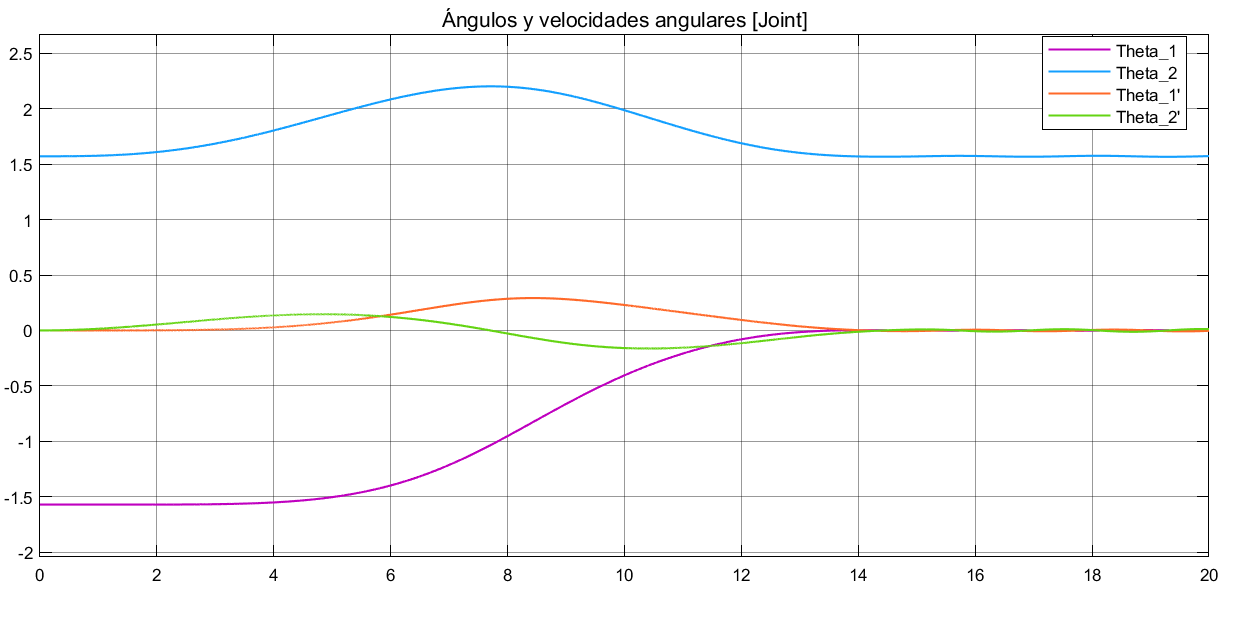
\includegraphics[width=0.8\linewidth]{ImagenesControl de posición no lineal/1_3_a}
	\caption{\'Angulos en funci\'on del tiempo en espacio joint.}	
	\label{fig:athetas}
\end{figure}
Aqu\'i se ven tanto las referencias como las coordendas reales que tomo el EE, con un error porcentual menor al XX$\%$ 
\begin{figure}[H]
	\centering
	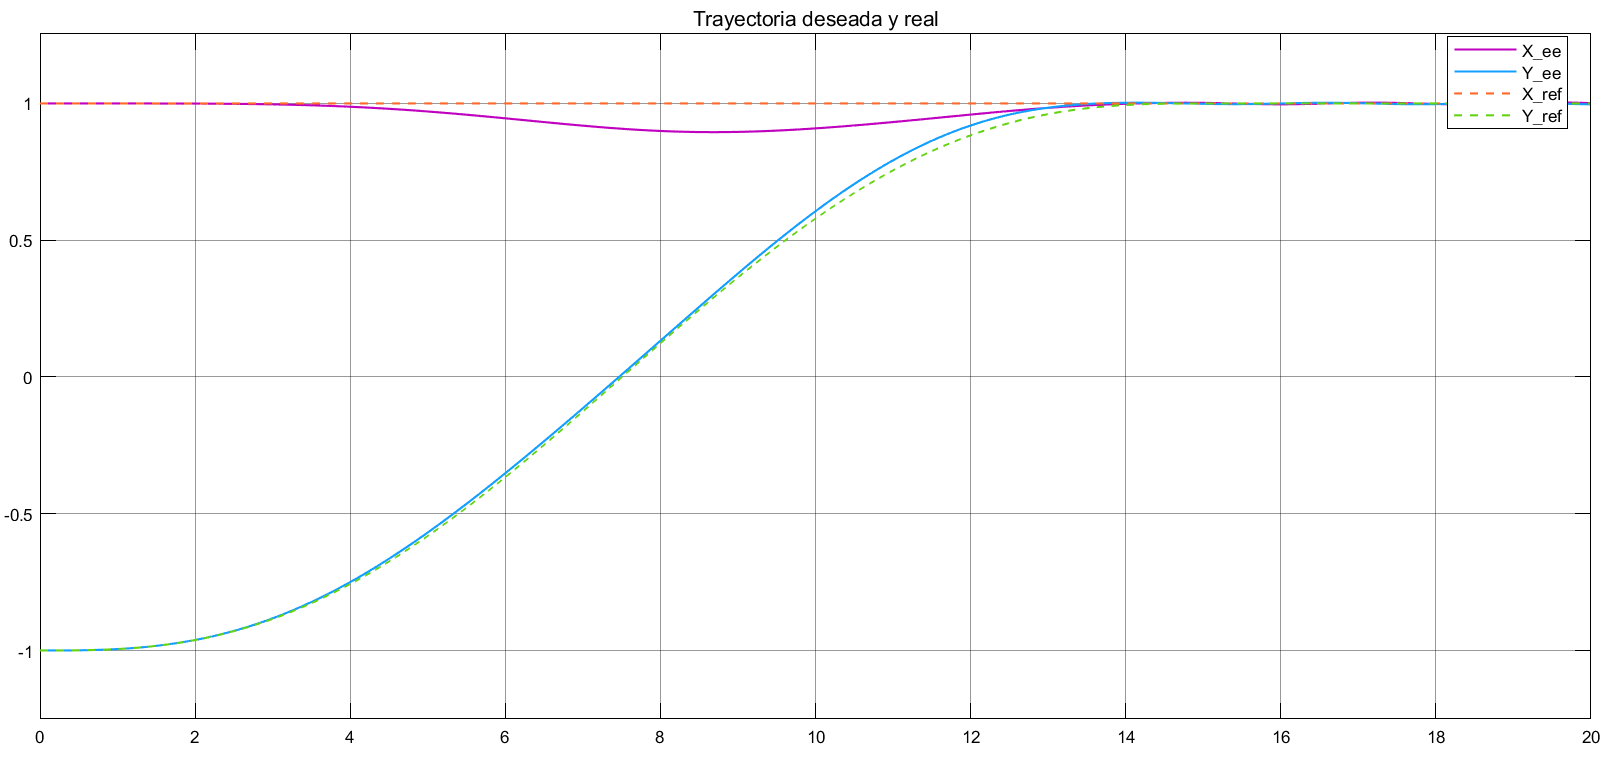
\includegraphics[width=0.8\linewidth]{ImagenesControl de posición no lineal/1_3_b}
	\caption{Posici\'on deseada y real del EE.}	
	\label{fig:apos}
\end{figure}

La trayectoria descripta por el EE se observa claramente en la siguiente imagen.
\begin{figure}[H]
	\centering
	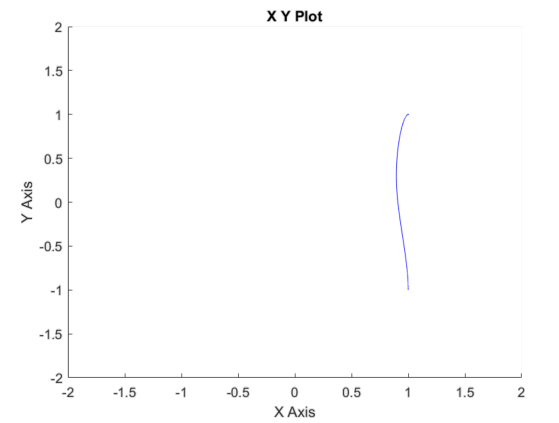
\includegraphics[width=0.5\linewidth]{ImagenesControl de posición no lineal/1_3_c}
	\caption{Gr\'afico XY.}	
	\label{fig:axy}
\end{figure}

Ademas se le incluy\'o un disturbio a la planta tanto en posici\'on como en velocidad. Este disturbio sucede en el segundo 14. Y se observa en los siguientes gráficos como el manipulador se ve afectado por el mismo y luego vuelve rápidamente a la referencia.

\begin{figure}[H]
	\centering
	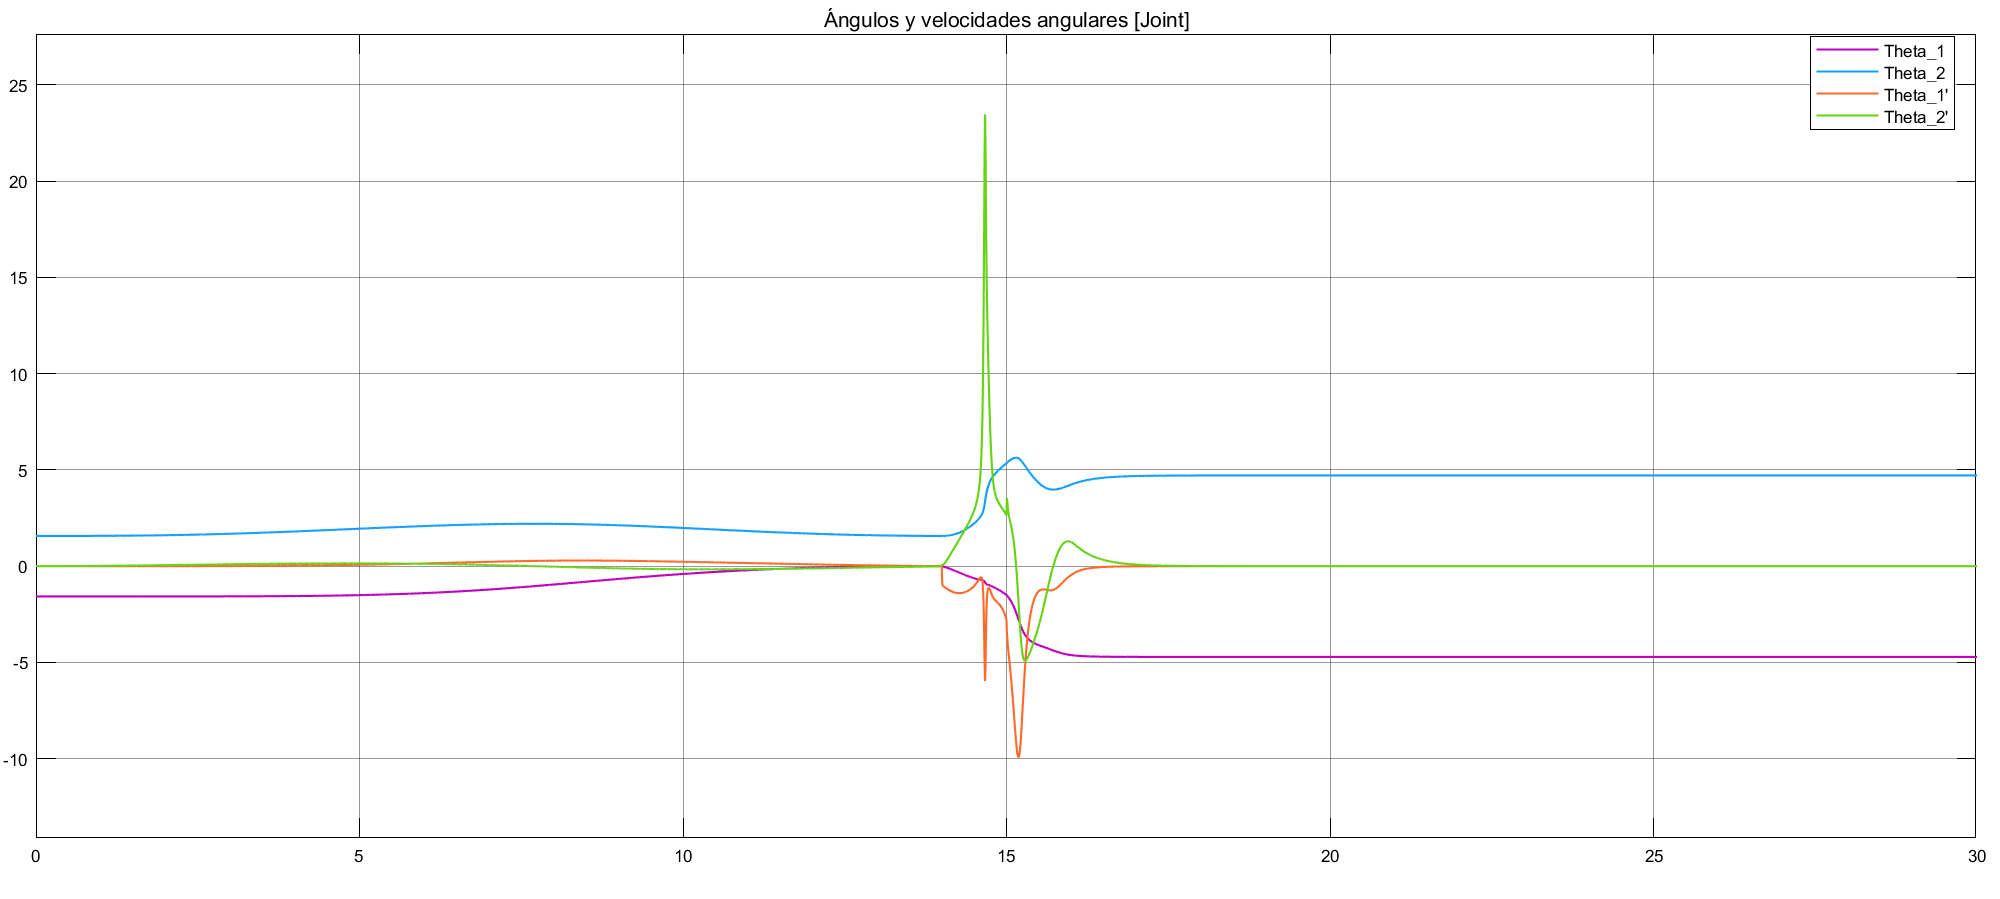
\includegraphics[width=0.8\linewidth]{ImagenesControl de posición no lineal/1_3_e_a}
	\caption{\'Angulos en funci\'on del tiempo en espacio joint.}	
	\label{fig:athetasd}
\end{figure}

\begin{figure}[H]
	\centering
	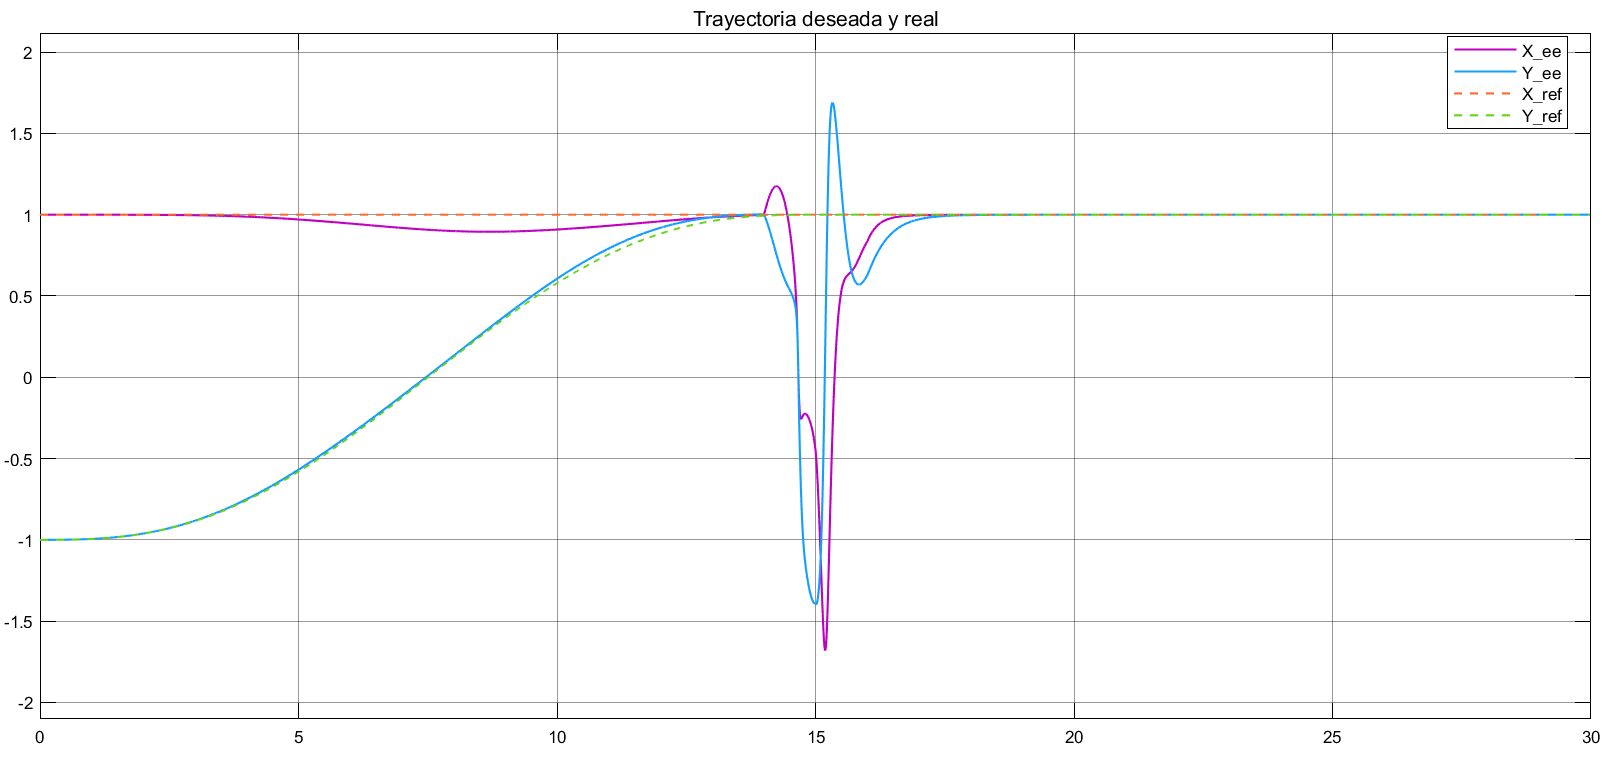
\includegraphics[width=0.8\linewidth]{ImagenesControl de posición no lineal/1_3_e_b}
	\caption{Posici\'on deseada y real del EE.}	
	\label{fig:aposd}
\end{figure}
\begin{figure}[H]
	\centering
	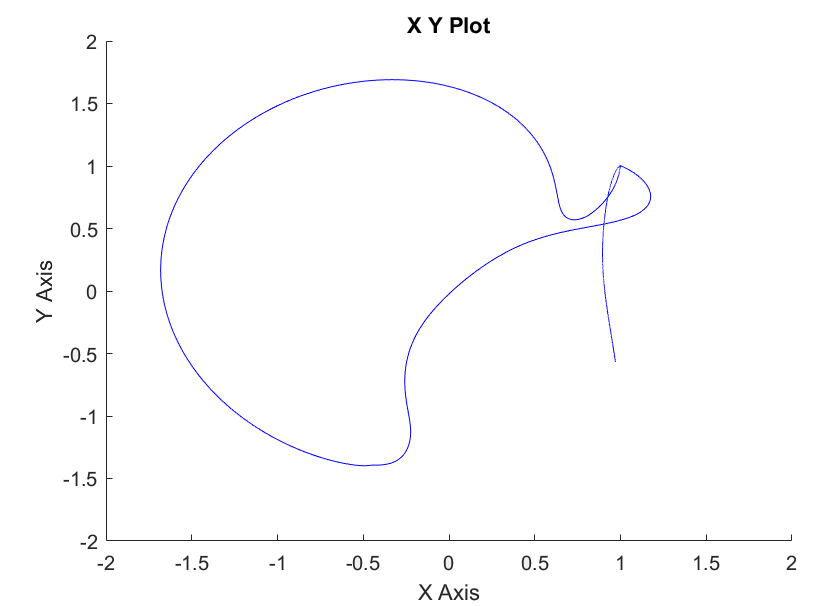
\includegraphics[width=0.5\linewidth]{ImagenesControl de posición no lineal/1_3_e_c}
	\caption{Gr\'afico XY.}	
	\label{fig:axyd}
\end{figure}

%\end{document}
